\documentclass[11pt]{article}
\usepackage{amsmath, amssymb, amscd, amsthm, amsfonts}
\usepackage{graphicx}
\usepackage{hyperref}
\usepackage{commath}
\usepackage{subfig}
\usepackage{float}
\usepackage{natbib}
\usepackage{booktabs}
\usepackage[toc,page]{appendix}
\oddsidemargin 0pt
\evensidemargin 0pt
\marginparwidth 40pt
\marginparsep 10pt
\topmargin -20pt
\headsep 10pt
\textheight 8.7in
\textwidth 6.65in
\linespread{1.5}

\title{Economics Influence on Housing price Index within Southeast Asian Countries}
\author{Steven Qin\\20819760\\s45qin@uwaterloo.ca \and Tiankai Jiang\\20834939\\t57jiang@uwaterloo.ca}

\date{\today}

\newtheorem{theorem}{Theorem}
\newtheorem{lemma}[theorem]{Lemma}
\newtheorem{conjecture}[theorem]{Conjecture}

\newcommand{\rr}{\mathbb{R}}

\newcommand{\al}{\alpha}
\DeclareMathOperator{\conv}{conv}
\DeclareMathOperator{\aff}{aff}

\makeatletter
\setlength{\@fptop}{0pt}
\makeatother

\begin{document}

\maketitle

\section{Introduction}\label{introduction}
TODO

\section{Literature Review}\label{literature_review}
This section reviews literature that focused on the relationship between housing price and macroeconomic factors. Some of the literature concentrated on macroeconomic factors, while others emphasized various analyzing techniques. Most of the papers concluded with several variables that they found could be the key factors that impact the housing price. The results are shown in the table \ref{literature_review}.

\begin{table}[H]
\begin{tabular}{|l|l|}
\hline
Author(s) (year)       & Macroeconomic Factors                                                                                                                                                                                                                     \\ \hline
\citet{aei297454}              & Mortgage loans, interest rates,  GDP, inflation rate                                                                                                                                                                                      \\ \hline
\citet{GASPARENIENE2016122}    & Availability of bank loans, interest rate, inflation rate, GDP                                                                                                                                                                            \\ \hline
\citet{GUPTA20112013}          & \begin{tabular}[c]{@{}l@{}}10 variables in \citet{10.1257/mac.2.2.125}, \\ 110 additional variables from \citet{10.1257/aer.99.1.350}\end{tabular}                                                                                                 \\ \hline
\citet{PAN20131720}            & \begin{tabular}[c]{@{}l@{}}Personal income growth rate, income \\ and labor force growth, bank instability\end{tabular}                                                                                                            \\ \hline
\citet{10.2307/23606731}       & Shocks on GDP, CPI, interest rate                                                                                                                                                                                                         \\ \hline
\citet{BELTRATTI2010533}       & \begin{tabular}[c]{@{}l@{}}GDP, private consumption and investment, CPI inflation, \\ short-and long-term interest rates\end{tabular}                                                                                                     \\ \hline
\citet{RePEc:pra:mprapa:98089} & \begin{tabular}[c]{@{}l@{}l@{}l@{}}Price-to-income ratio, price-to-rent ratio, urbanization,\\per-capita GDP, rent, inflation, GDP growth rate,\\ broad money, real exchange rate, percentage share\\of employment in services\end{tabular} \\ \hline
\citet{BOUCHOUICHA20121820}    & \begin{tabular}[c]{@{}l@{}}Inflation rate, short-and long-term interest rates, \\employment rate, money supply\end{tabular}                                                                                                              \\ \hline
\citet{PropertyPriceEurope}    & \begin{tabular}[c]{@{}l@{}l@{}}Unemployment rate, population growth,\\consumption expenditure, household consumption\\expenditure and housing expenses\end{tabular}                                                                          \\ \hline
\end{tabular}
\caption{Macroeconomic factors that have the impact on housing price level.}
\label{tab:literature_review}
\end{table}
\citet{aei297454} proposed a joint model to address the relationship between residential property price and several macro-economy indicators (e.g. mortgage loans, interest rates, the GDP, and inflation rate), aiming to forecast both the housing price and the economy in Belgium. Their approach is to use a dynamic factor model estimated with maximum likelihood and the EM algorithm, in which they assume that HPI and other macroeconomic variables comove strongly. They assume HPI can be modeled as a sum of two components: a ``common component'' that is driven by an unobserved factor such as business cycle, and an ``idiosyncratic component'' that is uncorrelated with the common component. Their result shows that the prediction over 2008q1-2009q4 was relatively accurate during 2008 while it underestimated quarterly growth rates in 2009. The authors state that at this stage, it is still a reduced-form exercise, and future works should focus on the discovery of shocks and their impact on the HPI forecast.

\citet{GASPARENIENE2016122} discussed the macroeconomic factors and house price level in Lithuania. The authors first summarized factors that could influence the house price from 14 previous papers, including GDP, employment rate, interest rate, and construction price, etc. Then, linear regression and methods for correlation were performed, accessing the impact of those factors on the average price of two-room apartments in Lithuania from 2008 to 2015. The result shows that the availability of bank loans and interest rate account most for the house price level, explain the variation of the house price by 79.03\% and 49.23\%, the inflation rate explains the price by 39.35\%, and GDP has the most insignificant impact amount these four variables in Lithuania.

\citet{10.2139/ssrn.2431627} stated that the issue among most house price forecasting models is that almost all time-series are aggregations of rather volatile elements, which introducing great error and making it difficult to generate an accurate model. In the paper, a three-step forecasting methodology was proposed to address this issue. First, a new method called Ensemble Empirical Mode Decomposition (EEMD) was used to smooth the original series data. Then, desired variables were selected using the Elastic Net approach. Finally, a Support Vector Regression model was constructed for forecasting. Using HPI data from 1989 to 2012 in the US, the result shows that their model outperforms all competing models in both in-sample and out-of-sample forecasting, and the model can make early accurate detection of the 2006-2009 price downturn.

\citet{GUPTA20112013} compared several time series models for HPI forecasting including dynamic stochastic general equilibrium (DSGE) model and the variations of vector autoregressive (VAR) models, such as Bayesian VAR (BVAR) models, Bayesian factor augmented VAR (BFAVAR), and small- and large-scale BVAR (SBVAR and LBVAR) models. 0 to 120 macro-economy factors are being used in different models to predict the HPI in the US. Using the period of 1976q1 to 2000q4 as the in-sample period and 2001q1 to 2005q2 as the out-of-sample horizon, they found that each model performs better in different periods and different conditions. They conjecture that the utilization of fundamental economic variables may improve the forecasting performance over models that do not use such data. But the gains do not prove statistically significant. Therefore, additional research is required.

Inspired by the subprime mortgage crisis developed in 2007 and 2008, which was triggered by the 2005 housing bubble burst, \citet{PAN20131720} investigate the relationship between the bank stability and the house prices in the US. Factors such as non-performing loans, equity ratio, cost-income ratio, and return on assets were selected. A threshold model was applied in the experiment. Their result shows that the personal income growth rate is considered as the threshold variable which interacts with the house price indicators in the threshold models. And the house price increase with rising demand due to income and labor force growth. The result also indicated a negative correlation between bank stability and house price.

\citet{10.2307/23606731} assessed the linkages between money, credit, house prices, and economic activity in industrialized countries between 1973q1 and 2006q4. The analysis was performed on 17 industrialized countries based on a fixed-effects panel vector autoregressive (VAR) model. The result found that money growth influences house prices and credit, credit influences money, and house prices and house prices influence both credit and money. Also, it is found that shocks on GDP, CPI, and interest rate have a significant effect on house prices, indicating that the linkages between those factors are all bidirectional. However, this result also indicates that the choice of predictors in regression analysis and predictions should be carefully selected since all factors are correlated.

\citet{BELTRATTI2010533} aimed to explore the linkages between general macroeconomic conditions and the housing market and whether there is a feedback effect of housing price shocks on the real economy. A Factor-Augmented Vector Autoregressive (F-VAR) model is used. The paper discussed the effect of eleven macroeconomic variables, including GDP, private consumption and investment, CPI inflation, short-and long-term interest rates, etc., on the housing price. The result shows that for G-7 countries, global macroeconomic shocks account for about 40\% in determining common house price fluctuations; productivity shocks are more important than demand shocks in determining house prices and the real estate itself accounts for about 20\% of the house price fluctuation.

While most previous research focused on the house price in one country, \citet{RePEc:pra:mprapa:98089} investigated the appropriate macroeconomic determinants of real house prices for 43 countries in the world from 1970 to 2017. The authors performed an OLS regression on the housing price. The result indicates that the price-to-income ratio, price-to-rent ratio, urbanization, per-capita GDP, rent, inflation, GDP growth rate, broad money, and real exchange rate influence positively on housing prices. The percentage share of employment in services influence negatively on real house prices. Finally, there is not enough evidence to show the real interest rate affects the housing price. The target countries are separated into four groups based on their income, just like what we did in this paper. The author also found a gap between countries with different income levels, suggesting that the gap was mainly caused by urbanization and different regulation of housing prices in those countries.

\citet{BOUCHOUICHA20121820} used dynamic coherence function (DCF), which was proposed by \citet{10.2307/2984905}, to analyze the real estate time series data of the UK and the US market. And they chose inflation rate, short-and long-term interest rates, employment rate, and money supply as the macroeconomic data. They found some synchronization between the UK and the US real estate markets in their long-run co-movements with the long-term interest rate, inflation, and employment rate. However, they also found desynchronization between the two countries in terms of economic growth, the money supply, and the short-term interest rate, which provided suggestions when selecting the independent variables in regression analysis, especially when comparing different countries' real estate data within the same time frame.

Finally, \citet{PropertyPriceEurope} presented Artificial Neural Networks (ANN) model to select macroeconomic factors that could affect real estates. They chose 14 macroeconomic factors (e.g. GDP, unemployment rate, CPI...) as alternative independent variables and the house price index in Poland and Italy as dependent variables. Although ANN will not be used in this paper, it is usually provided with high accuracy and its result could be referred to as we choosing independent variables. They found for the developing country, i.e. Poland, unemployment rate, and population growth are the key factors that influence the house price. Whereas for a developed country, i.e. Italy, consumption expenditure, household consumption expenditure, and housing expenses have a major effect on the house price.

\section{Methods}\label{methods}
In this section, we will first talk about the candidate independent variables, their relationship with annual HPI and why do we select them. Then, the mathematical model will be proposed. Finally, since there are too many candidate variables, a reliable method will be proposed to filter those variables.

\subsection{Variables}\label{variables}
TODO

\subsection{Model Description}\label{model_description}
There are three methods mentioned in section \ref{literature_review} to analyze and predict annual HPI data, namely, linear regression, time series analysis, and artificial neural network. We chose to use linear regression, like the one that was used in \citet{GASPARENIENE2016122}. The model is shown as follows:
$$y = \beta_0 + \beta_1x_1 + \beta_2x_2 + ... + \beta_nx_n + \epsilon$$
in which $y$ represents the annual HPI and each $x$ could be a candidate variable. The $\beta$s are the values we desire in the regression.

The reason we chose linear regression instead of the other two methods is that those two methods require a lot more data. Generally, all papers that did not use linear regression used data from the 1970s to 2010s. However, we only have 11 years of data on annual HPI, which is insufficient to perform those analyses. Also, as mentioned in section \ref{introduction}, we want to build a unified model for all four countries, which means we want to find the same independent variables for all four countries. Implementing a Vector Autoregressive model is too complicated for that.

\subsection{Variables Selection}\label{variables_selection}
We have mentioned in the previous section that there are lots of independent variables that may influence the house price index. It is obvious that we cannot use all of them for regression. Therefore, the first step is to select the proper independent variables. We have the following constraints:
\begin{enumerate}
    \item It is not possible to fit all four countries in the same linear function with the same coefficients, however, we should at least use the same independent variables for four regressions. Otherwise, the results are just four separate models without comparability.
    \item When selecting the independent variables for regression, any selected variable should be strongly correlated with HPI.
    \item When selecting the independent variables for regression, all selected variables should not be strongly correlated with each other.
\end{enumerate}
Our strategy is\citep{Feature}:
\begin{enumerate}
    \item We construct the Pearson Correlation Table of all variables for all four countries. And remove a variable if, in any tables, the correlation between that variable and the annual HPI is less or equal to 0.5.
    \item After the first step, all variables left are strongly correlated with annual HPI. We construct the Pearson Correlation Table again, this time, for all independent variables left. And we only pick one from a group, if that group of variables is strongly correlated with each other (here we pick r=0.7). 
\end{enumerate}

We use China as an example, below is the Pearson Correlation Table constructed in step 1. Here actually we only use the annual HPI row (indicate by a green arrow):
\begin{figure}[H]
\begin{center}
    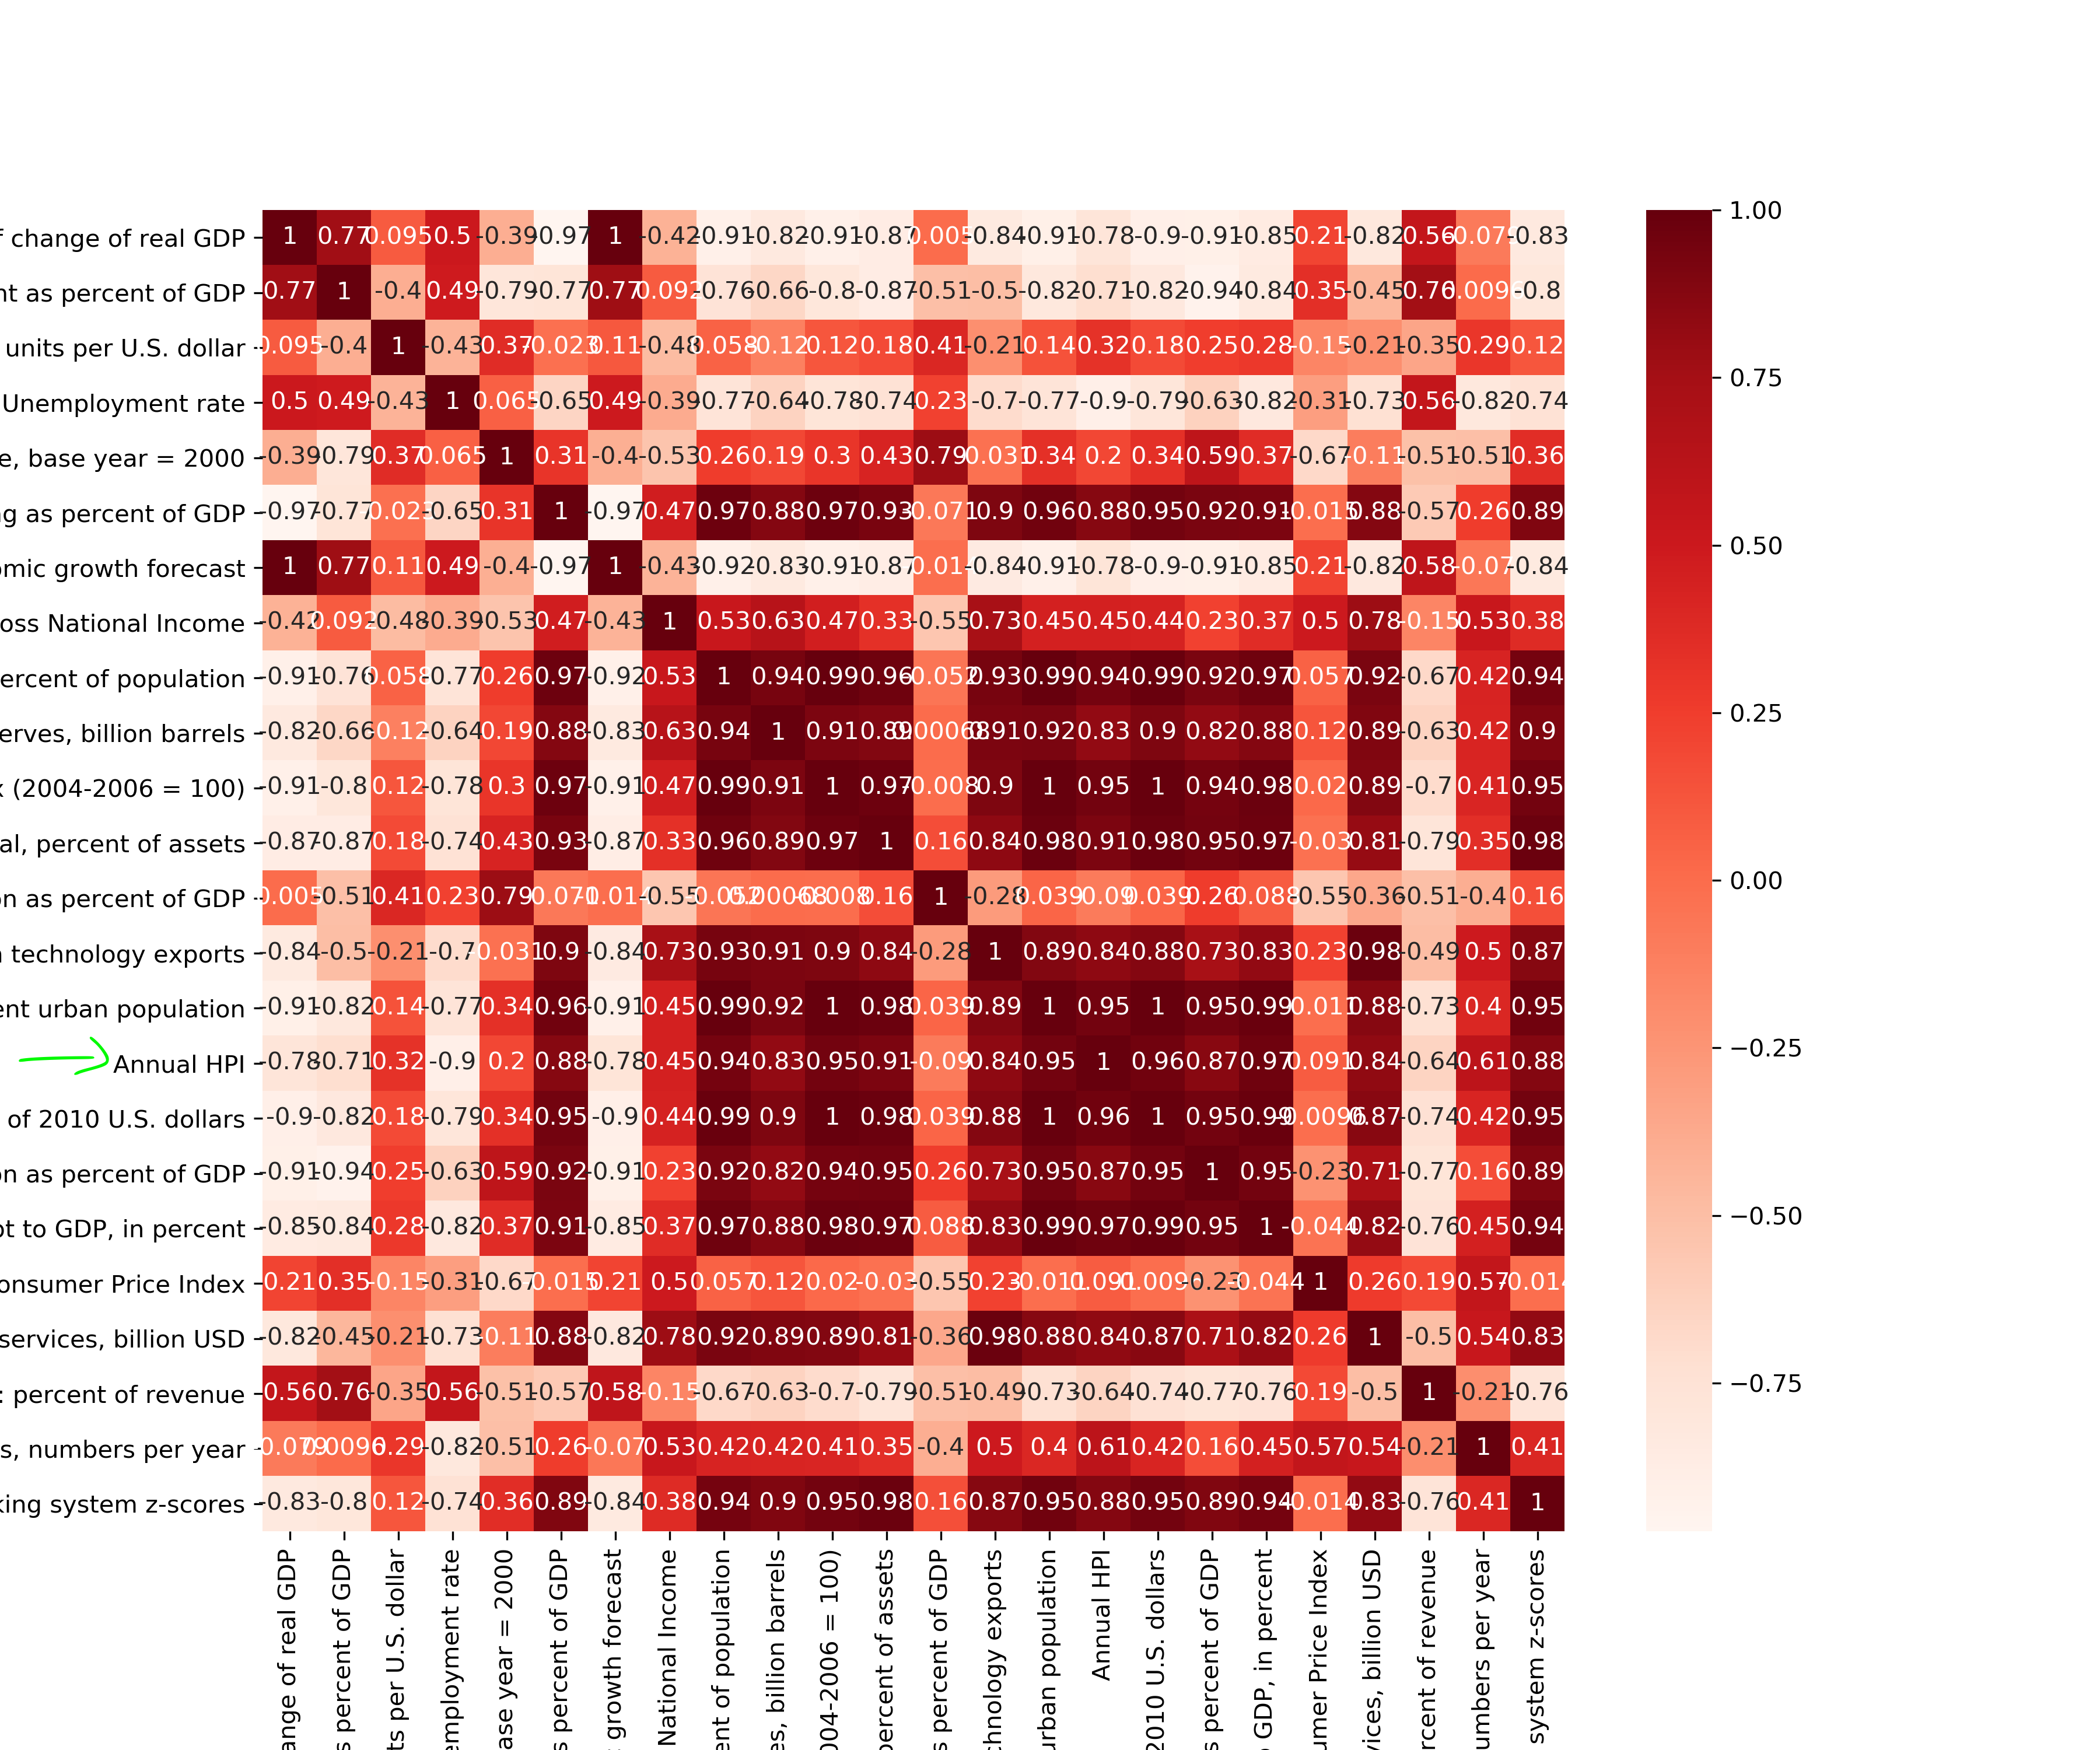
\includegraphics[width=1.0\textwidth]{./image/CorrelationTable1.png}
\end{center}
\end{figure}
After doing this step for all four countries, we plot the correlation table for all variables left:
\begin{figure}[H]
\begin{center}
    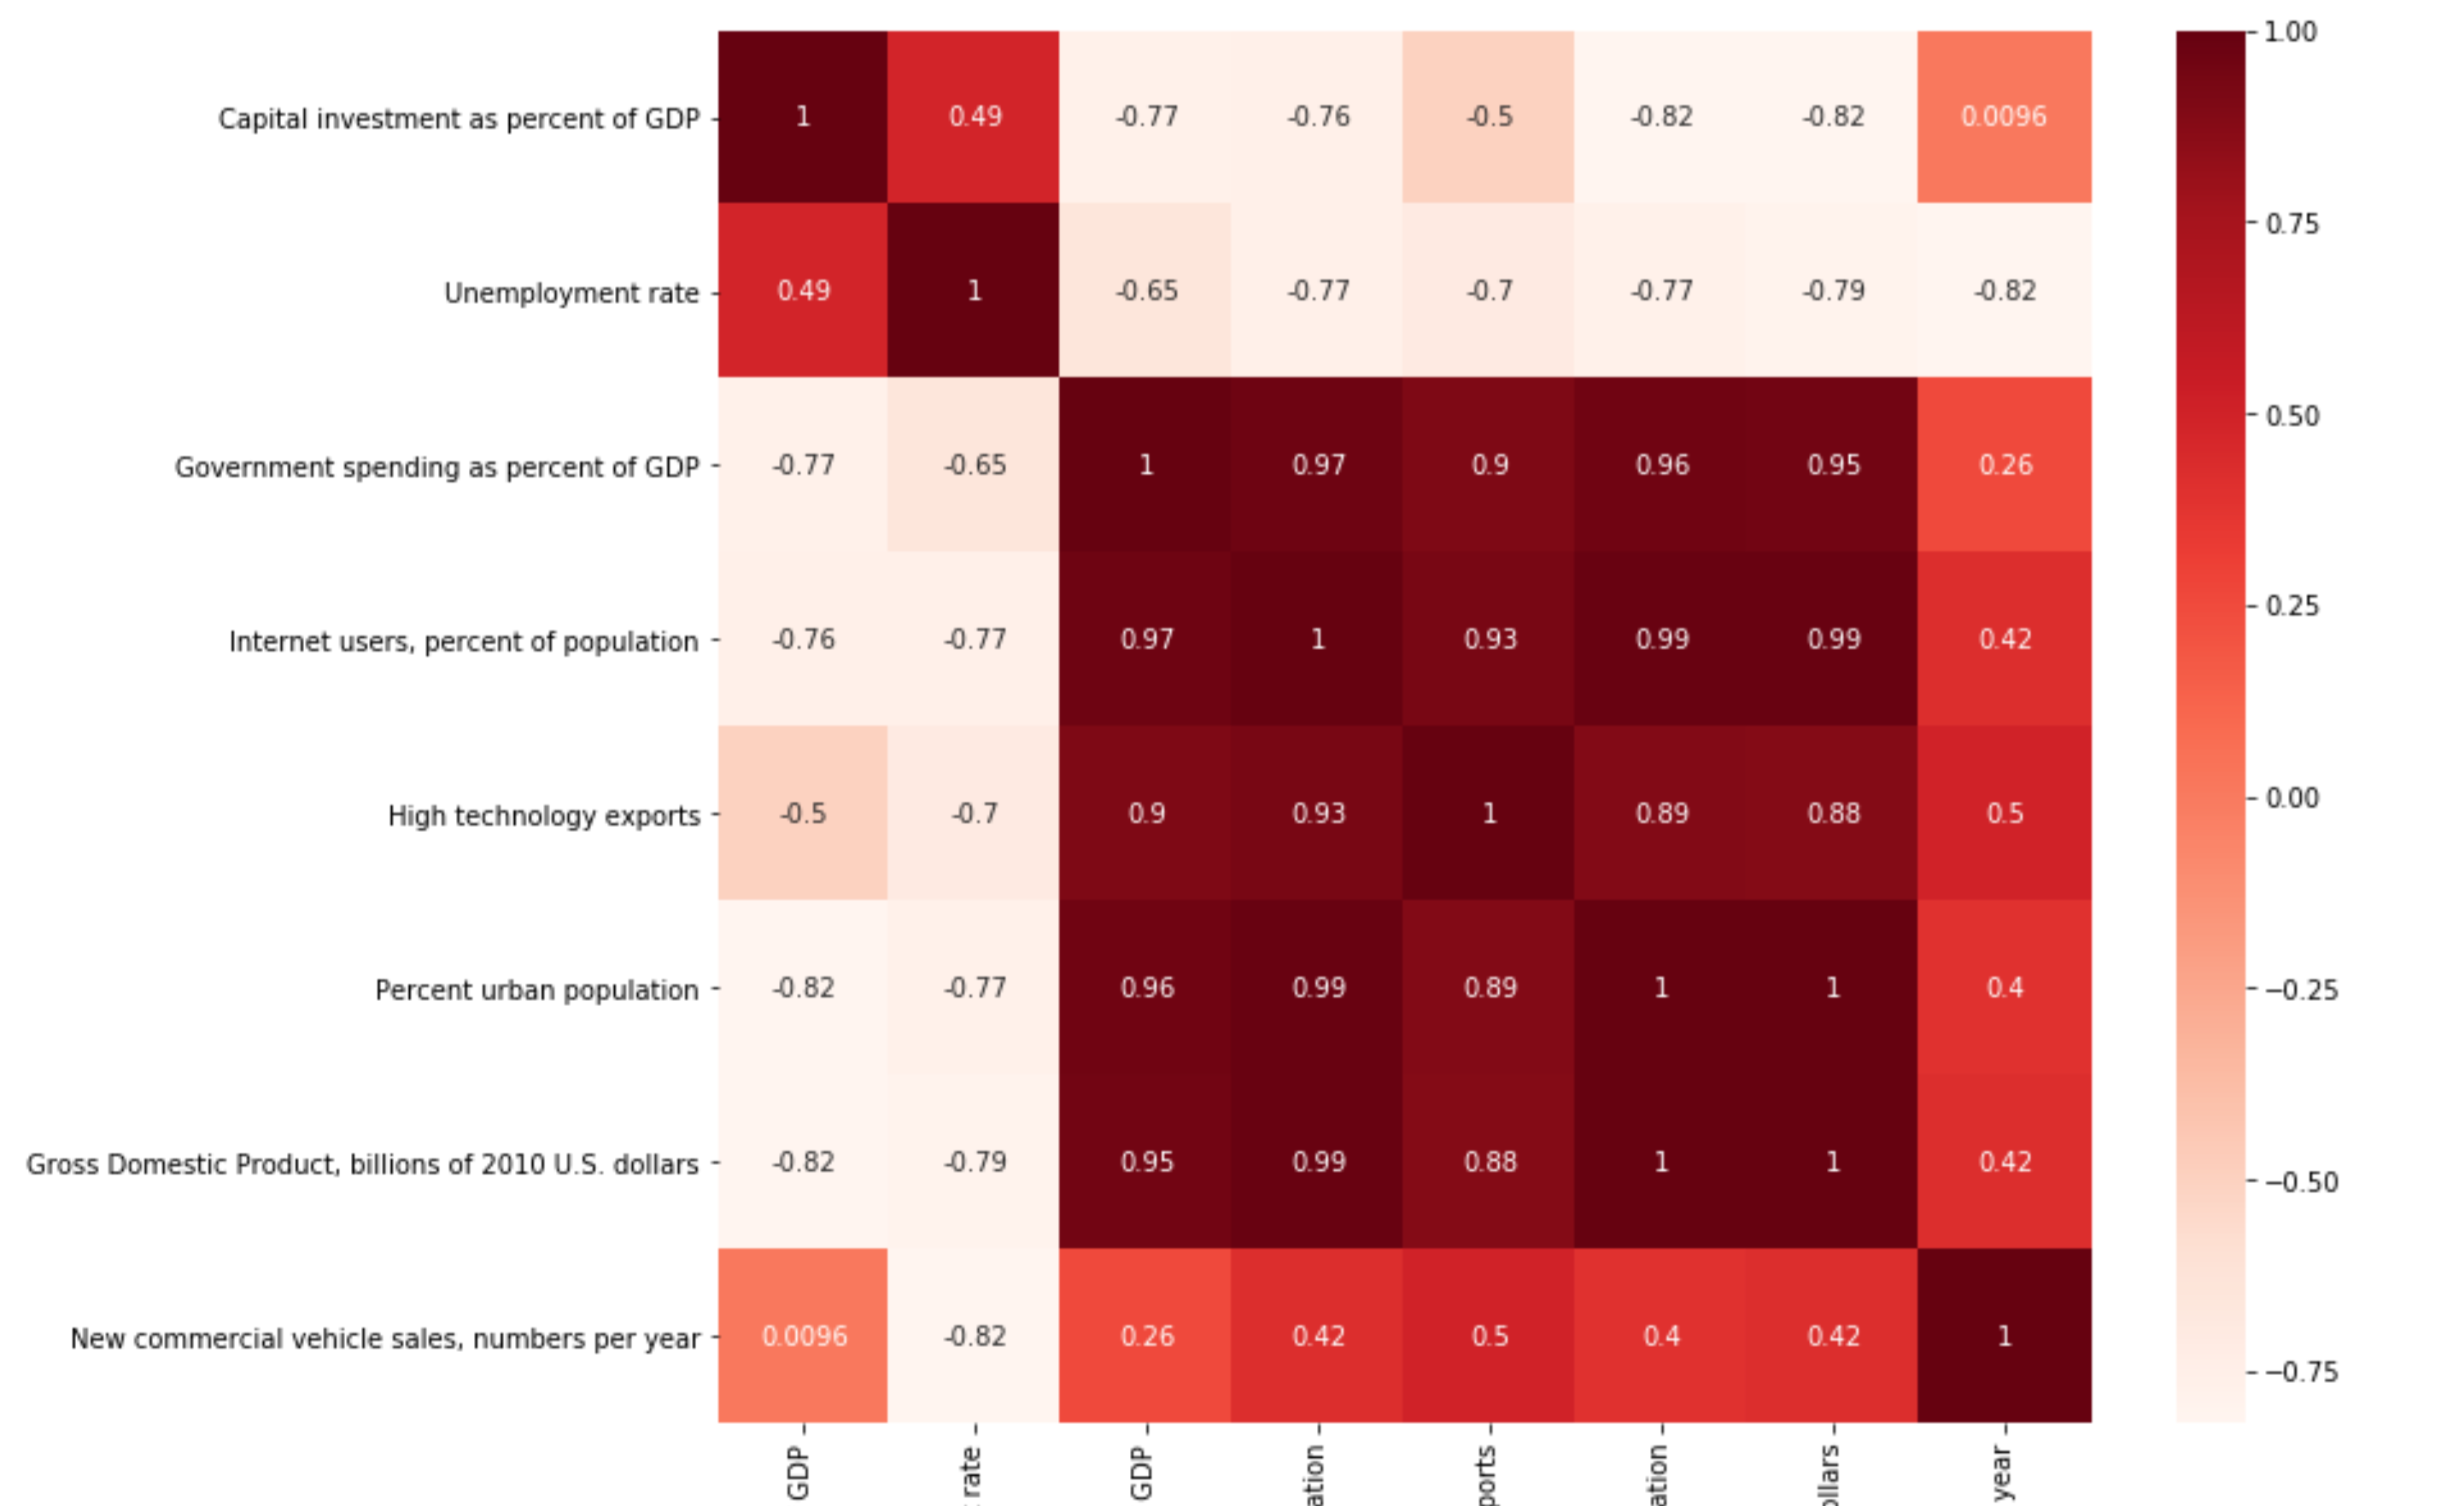
\includegraphics[width=1.0\textwidth]{./image/CorrelationTable2.png}
\end{center}
\end{figure}
Lots of independent variables are strongly correlated, which does not satisfy the assumption of linear regression. Based on the results mentioned in the literature reviews, here we pick only the Unemployment rate and Government spending as percent of GDP (row 2 and row 3).

\section{Data}\label{data}
We chose annual HPI as our dependent variable and based on the previous research, we chose 23 candidate variables for regression analysis. The relationship between those candidate variables and the annual HPI has been discussed in section \ref{methods}. The appendix contains a description of each variable, its type, how it was constructed, and the data source. The table below shows the mean, standard deviation, minimum, and maximum of each variable. We group the result by countries.
\begin{table}[H]
\begin{tabular}{lrrrr}
\toprule
{} Variable&        mean &        std &         min &         max \\
\midrule
Economic growth: the rate of change of real GDP    &       0.673 &      2.353 &      -5.420 &       4.190 \\
Capital investment as percent of GDP               &      23.025 &      1.130 &      21.300 &      24.320 \\
Exchange rate: local currency units per U.S. do... &     100.538 &     13.793 &      79.790 &     121.040 \\
Unemployment rate                                  &       3.692 &      0.999 &       2.290 &       5.100 \\
Terms of trade, base year = 2000                   &      65.403 &      5.525 &      58.440 &      74.370 \\
Government spending as percent of GDP              &      19.893 &      0.262 &      19.490 &      20.250 \\
Economic growth forecast                           &       0.672 &      2.353 &      -5.420 &       4.190 \\
Internet users, percent of population              &      85.934 &      6.391 &      78.000 &      93.180 \\
Oil reserves, billion barrels                      &       0.040 &      0.000 &       0.040 &       0.040 \\
Crop production index (2004-2006 = 100)            &      91.250 &      4.264 &      81.800 &      96.700 \\
Banking system capital, percent of assets          &       5.270 &      0.412 &       4.300 &       5.630 \\
Stock market capitalization as percent of GDP      &      89.781 &     26.454 &      54.010 &     127.860 \\
High technology exports                            &  112398.783 &  12738.820 &   98537.260 &  133518.230 \\
Percent urban population                           &      91.205 &      0.478 &      89.990 &      91.700 \\
Gross Domestic Product, billions of 2010 U.S. d... &    5908.509 &    231.440 &    5470.800 &    6210.700 \\
Household consumption as percent of GDP            &      57.198 &      1.461 &      55.339 &      58.960 \\
Household debt to GDP, in percent                  &      53.427 &     17.807 &       0.000 &      62.500 \\
Inflation: percent change in the Consumer Price... &       0.300 &      1.079 &      -1.400 &       2.800 \\
Imports of goods and services, billion USD         &     852.938 &    119.272 &     626.200 &     998.180 \\
Income, profits, and capital gains taxes: perce... &      47.820 &      2.358 &      42.110 &      50.960 \\
New commercial vehicle sales, numbers per year     &  809939.636 &  65941.198 &  701188.000 &  894125.000 \\
Banking system z-scores                            &      15.349 &      2.031 &      10.330 &      18.013 \\
\bottomrule
\end{tabular}
\caption{Mean, Standard deviation, Min and Maximum of each variable, Japan}
\label{tab:describe_jpn}
\end{table}

\begin{table}[H]
\begin{tabular}{lrrrr}
\toprule
{} Variable&         mean &         std &          min &          max \\
\midrule
Economic growth: the rate of change of real GDP    &        7.849 &       1.413 &        6.110 &       10.640 \\
Capital investment as percent of GDP               &       44.761 &       1.685 &       42.630 &       46.660 \\
Exchange rate: local currency units per U.S. do... &        6.534 &       0.277 &        6.140 &        6.910 \\
Unemployment rate                                  &        4.525 &       0.131 &        4.280 &        4.720 \\
Terms of trade, base year = 2000                   &       85.492 &       5.045 &       79.050 &       92.530 \\
Government spending as percent of GDP              &       15.854 &       0.736 &       14.590 &       16.919 \\
Economic growth forecast                           &        7.820 &       1.404 &        6.110 &       10.560 \\
External debt, percent of Gross National Income    &       13.532 &       2.100 &        8.920 &       16.950 \\
Internet users, percent of population              &       47.054 &      10.472 &       28.900 &       62.712 \\
Oil reserves, billion barrels                      &       22.919 &       3.194 &       16.000 &       25.930 \\
Crop production index (2004-2006 = 100)            &      137.225 &      12.943 &      116.800 &      156.683 \\
Banking system capital, percent of assets          &        7.448 &       1.282 &        5.600 &        9.341 \\
Stock market capitalization as percent of GDP      &       58.013 &      12.249 &       41.260 &       74.020 \\
High technology exports                            &   606382.805 &  114654.551 &   359273.920 &   759591.883 \\
Percent urban population                           &       54.210 &       4.120 &       47.880 &       60.310 \\
Gross Domestic Product, billions of 2010 U.S. d... &     8414.664 &    1982.378 &     5502.000 &    11537.200 \\
Household consumption as percent of GDP            &       36.858 &       1.790 &       34.330 &       39.433 \\
Household debt to GDP, in percent                  &       37.790 &      10.745 &       23.500 &       53.793 \\
Inflation: percent change in the Consumer Price... &        2.291 &       1.511 &       -0.700 &        5.600 \\
Imports of goods and services, billion USD         &     1980.514 &     437.674 &     1042.530 &     2548.880 \\
Income, profits, and capital gains taxes: perce... &       22.371 &       3.175 &       18.864 &       28.270 \\
New commercial vehicle sales, numbers per year     &  3933418.000 &  359135.486 &  3313479.000 &  4370795.000 \\
Banking system z-scores                            &       20.852 &       2.269 &       17.130 &       24.116 \\
\bottomrule
\end{tabular}
\caption{Mean, Standard deviation, Min and Maximum of each variable, China}
\label{tab:describe_chn}
\end{table}

\begin{table}[H]
\begin{tabular}{lrrrr}
\toprule
{} Variable&        mean &        std &       min &        max \\
\midrule
Economic growth: the rate of change of real GDP    &       5.950 &      1.759 &      1.45 &       7.33 \\
Capital investment as percent of GDP               &      22.235 &      3.120 &     17.43 &      27.15 \\
Exchange rate: local currency units per U.S. do... &      46.639 &      3.682 &     42.23 &      52.66 \\
Unemployment rate                                  &       3.135 &      0.598 &      2.15 &       3.86 \\
Terms of trade, base year = 2000                   &      79.358 &      3.932 &     73.52 &      84.20 \\
Government spending as percent of GDP              &      10.863 &      0.913 &      9.71 &      12.53 \\
Economic growth forecast                           &       5.951 &      1.760 &      1.45 &       7.34 \\
External debt, percent of Gross National Income    &      23.135 &      3.074 &     20.13 &      28.49 \\
Internet users, percent of population              &      39.152 &     15.417 &      9.00 &      60.05 \\
Oil reserves, billion barrels                      &       0.140 &      0.000 &      0.14 &       0.14 \\
Crop production index (2004-2006 = 100)            &     114.112 &      3.567 &    109.60 &     119.30 \\
Banking system capital, percent of assets          &      10.213 &      0.719 &      9.50 &      11.70 \\
Stock market capitalization as percent of GDP      &      76.018 &     10.980 &     49.03 &      88.41 \\
High technology exports                            &   33703.015 &    283.599 &  33502.48 &   33903.55 \\
Percent urban population                           &      46.128 &      0.625 &     45.33 &      47.15 \\
Gross Domestic Product, billions of 2010 U.S. d... &     269.055 &     55.812 &    194.10 &     360.90 \\
Household consumption as percent of GDP            &      72.208 &      0.859 &     70.19 &      73.21 \\
Household debt to GDP, in percent                  &       0.000 &      0.000 &      0.00 &       0.00 \\
Inflation: percent change in the Consumer Price... &       3.136 &      1.363 &      0.70 &       5.20 \\
Imports of goods and services, billion USD         &      98.596 &     31.768 &     54.01 &     151.72 \\
Income, profits, and capital gains taxes: perce... &      40.729 &      1.716 &     36.53 &      42.08 \\
New commercial vehicle sales, numbers per year     &  142465.909 &  38579.063 &  86333.00 &  226384.00 \\
Banking system z-scores                            &      18.112 &      1.127 &     16.19 &      20.71 \\
\bottomrule
\end{tabular}
\caption{Mean, Standard deviation, Min and Maximum of each variable, Philippines}
\label{tab:describe_phl}
\end{table}

\begin{table}[H]
\begin{tabular}{lrrrr}
\toprule
{} Variable&        mean &         std &        min &          max \\
\midrule
Economic growth: the rate of change of real GDP    &       6.845 &       1.266 &       5.02 &        8.500 \\
Capital investment as percent of GDP               &      34.689 &       4.111 &      30.17 &       40.220 \\
Exchange rate: local currency units per U.S. do... &      59.015 &       9.084 &      45.73 &       70.420 \\
Unemployment rate                                  &       5.543 &       0.121 &       5.33 &        5.670 \\
Terms of trade, base year = 2000                   &      97.596 &       6.501 &      89.99 &      108.190 \\
Government spending as percent of GDP              &      10.847 &       0.483 &      10.30 &       11.770 \\
Economic growth forecast                           &       7.113 &       1.644 &       4.18 &       10.260 \\
External debt, percent of Gross National Income    &      20.443 &       1.949 &      17.52 &       23.300 \\
Internet users, percent of population              &      17.412 &       8.497 &       5.12 &       32.000 \\
Oil reserves, billion barrels                      &       5.235 &       0.539 &       4.42 &        5.680 \\
Crop production index (2004-2006 = 100)            &     140.275 &      13.405 &     112.80 &      159.317 \\
Banking system capital, percent of assets          &       7.108 &       0.205 &       6.70 &        7.390 \\
Stock market capitalization as percent of GDP      &      76.156 &      13.504 &      55.25 &       97.390 \\
High technology exports                            &   15466.125 &    3058.267 &   10778.73 &    20273.090 \\
Percent urban population                           &      32.443 &       1.287 &      30.59 &       34.470 \\
Gross Domestic Product, billions of 2010 U.S. d... &    2197.400 &     483.493 &    1544.40 &     2964.000 \\
Household consumption as percent of GDP            &      57.820 &       1.755 &      54.72 &       60.240 \\
Household debt to GDP, in percent                  &       9.841 &       0.838 &       8.90 &       11.300 \\
Inflation: percent change in the Consumer Price... &       7.664 &       3.010 &       2.50 &       12.000 \\
Imports of goods and services, billion USD         &     524.751 &      84.219 &     347.18 &      639.010 \\
Income, profits, and capital gains taxes: perce... &      44.837 &       2.997 &      41.25 &       50.270 \\
New commercial vehicle sales, numbers per year     &  730269.091 &  148067.419 &  449391.00 &  1005380.000 \\
Banking system z-scores                            &      16.813 &       0.470 &      15.96 &       17.560 \\
\bottomrule
\end{tabular}
\caption{Mean, Standard deviation, Min and Maximum of each variable, India}
\label{tab:describe_ind}
\end{table}

\section{Results}\label{results}
\subsection{Normality of the Dependent Variable}\label{normality_check}
Kolmolgorov-Smirnoff test was used to check normality of the dependent variable.
$$D=\underset{1 \leq i \leq N}{\max}(F(Y_i)-\frac{i-1}{N},\frac{i}{N}-F(Y_i))$$
$H_0$: The variable is normally distributed.\\
$H_a$: The variable is not normally distributed.\\
For China, India, Japan, Philippines, the result are \textbf{0.1873, 0.1224, 0.1338, 0.1536} respectively. According to the One-Sample Kolmogorov-Smirnov Table (Appendix \ref{kstable}), when $n=11$ and $\alpha=0.05$, the critical value $D_{n,a}=0.3912$. All four results are less than the critical value. Therefore, we failed to reject the $H_0$. The dependent variable is normally distributed.

\subsection{Mean Comparison of the Dependent Variable}\label{mean_comparison}
One-tail two sample independent t-test was performed on all four countries. Therefore, there are 6 comparisons in total.\\
Let $\mu_1$ denotes the average HPI of the country in the first column, $\mu_2$ denotes the average HPI of the country in the second column.\\
$H_0: \mu_1\geq \mu_2$\\
$H_a: \mu_1< \mu_2$\\
$df=11+11-2=20$, the critical value for an one-tail t-test when $\alpha=0.05$ is $t_{crit}=1.725$.\\
The results are shown in table \ref{tab:comparison_results}.
\begin{table}[H]
\begin{tabular}{|l|l|l|l|l|}
\hline
Country A   & Country B   & $t_{obj}$ & $t_{crit}$ & result \\ \hline
India       & Philippines & 1.395607763 & 0          & 0      \\ \hline
Philippines & China       & 2.481775986 & 0          & 1      \\ \hline
China       & Japan       & 2.196236113 & 0          & 1      \\ \hline
Philippines & Japan       & 3.070888374 & 0          & 1      \\ \hline
India       & China       & 3.929769778 & 0          & 1      \\ \hline
India       & Japan       & 4.449066711 & 0          & 1      \\ \hline
\end{tabular}
\caption{Comparison Results}
\label{tab:comparison_results}
\end{table}

For the comparison between India and Philippines, $t_{obj}=1.3956<t_{crit}$. We failed to reject $H_0$ and conclude that there is not enough evidence to show that the average HPI of Philippines is greater than that of India. For all other five comparisions, $t_{obj}>t_{crit}$, we reject $H_0$ and conclude that the HPI of the country in the second column is indeed greater than that in the first column.

\subsection{Regression and Residuals Analysis}\label{result_analysis}
The regression results are summarized in the table \ref{tab:regression_results}. 
\begin{table}[]
\renewcommand{\arraystretch}{0.8}
\begin{tabular}{lrrrr}
\toprule
                           &        Japan &        China & Philippines &        India \\
\midrule
                    Model: &          OLS &          OLS &         OLS &          OLS \\
       Dependent Variable: &   Annual HPI &   Annual HPI &  Annual HPI &   Annual HPI \\
         No. Observations: &           11 &           11 &          11 &           11 \\
                 Df Model: &            2 &            2 &           2 &            2 \\
             Df Residuals: &            8 &            8 &           8 &            8 \\
                R-squared: &        0.965 &        0.957 &       0.932 &        0.851 \\
           Adj. R-squared: &        0.956 &        0.946 &       0.914 &        0.814 \\
                      AIC: &      35.5778 &      59.7291 &     97.2204 &     109.2955 \\
                      BIC: &      36.7715 &      60.9228 &     98.4141 &     110.4891 \\
           Log-Likelihood: &      -14.789 &      -26.865 &     -45.610 &      -51.648 \\
              F-statistic: &        110.0 &        88.39 &       54.40 &        22.82 \\
       Prob (F-statistic): &     1.51e-06 &     3.51e-06 &    2.20e-05 &     0.000495 \\
                    Scale: &       1.1847 &       10.645 &      321.61 &       963.98 \\
               const\_Coef. &       229.38 &      238.571 &    -72.1933 &      4451.38 \\
            const\_Std.Err. &      26.1221 &      69.3646 &     243.306 &      649.735 \\
                   const\_t &      8.78105 &      3.43938 &   -0.296718 &      6.85107 \\
               const\_P$>\abs{t}$ &  2.22013e-05 &    0.0088319 &    0.774239 &  0.000130848 \\
    UnemploymentRate\_Coef. &     -4.85583 &     -61.1828 &    -47.3606 &     -607.825 \\
 UnemploymentRate\_Std.Err. &      0.34461 &      10.3284 &      24.161 &       90.384 \\
        UnemploymentRate\_t &     -14.0908 &     -5.92375 &     -1.9602 &     -6.72492 \\
    UnemploymentRate\_P$>\abs{t}$ &    6.251e-07 &  0.000352204 &   0.0856311 &  0.000148837 \\
         GovSpending\_Coef. &     -5.39993 &      9.59926 &     35.1322 &     -81.2761 \\
      GovSpending\_Std.Err. &      1.31389 &      1.84297 &     15.8131 &      22.7249 \\
             GovSpending\_t &     -4.10989 &      5.20857 &     2.22171 &     -3.57653 \\
         GovSpending\_P$>\abs{t}$&   0.00339113 &  0.000813845 &   0.0570298 &   0.00722465 \\
                  Omnibus: &        0.532 &        4.142 &       0.539 &        0.354 \\
            Prob(Omnibus): &        0.766 &        0.126 &       0.764 &        0.838 \\
                     Skew: &       -0.192 &       -0.954 &       0.401 &        0.241 \\
                 Kurtosis: &        1.985 &        3.319 &       2.385 &        2.642 \\
            Durbin-Watson: &        1.453 &        1.995 &       1.853 &        1.195 \\
         Jarque-Bera (JB): &        0.541 &        1.714 &       0.469 &        0.165 \\
                 Prob(JB): &        0.763 &        0.425 &       0.791 &        0.921 \\
            Condition No.: &         1615 &         1177 &         515 &          856 \\
\bottomrule
\end{tabular}
\caption{Regression Results}
\label{tab:regression_results}
\end{table}

\section{Implications and conclusion}\label{conclusion}

\newpage
\bibliographystyle{apalike}
\bibliography{references}

\begin{appendices}
\section{Data Source and Description}
All data in this paper is from \href{https://www.theglobaleconomy.com/download-data.php}{the Global Economy}.\\

\textbf{Economic growth: the rate of change of real GDP}: Annual percentage growth rate of GDP at market prices based on constant local currency. Aggregates are based on constant 2010 U.S. dollars. Type: Ratio.

\textbf{Capital investment as percent of GDP}: Gross capital formation (formerly gross domestic investment) consists of outlays on additions to the fixed assets of the economy plus net changes in the level of inventories. Type: Ratio.

\textbf{Exchange rate: local currency units per U.S. dollar}: Official exchange rate refers to the exchange rate determined by national authorities or to the rate determined in the legally sanctioned exchange market. It is calculated as an annual average based on monthly averages (local currency units relative to the U.S. dollar). Type: Ratio.

\textbf{Unemployment rate}: Unemployment refers to the share of the labor force that is without work but available for and seeking employment. Type: Ratio.

\textbf{Terms of trade}: Net barter terms of trade index is calculated as the percentage ratio of the export unit value indexes to the import unit value indexes, measured relative to the base year 2000. Type: Ratio.

\textbf{Government spending as percent of GDP}: General government final consumption expenditure (formerly general government consumption) includes all government current expenditures for purchases of goods and services (including compensation of employees). Type: Ratio.

\textbf{Economic growth forecast}: Year-on-year percent changes in constant price GDP. The base year is country-specific. Type: Ratio.

\textbf{External debt, percent of Gross National Income}: Total external debt stocks to gross national income. Total external debt is debt owed to nonresidents repayable in currency, goods, or services. Type: Ratio.

\textbf{Internet users, percent of population}: Internet users are individuals who have used the Internet (from any location) in the last 3 months. Type: Ratio.

\textbf{Oil reserves, billion barrels}: Proved reserves of crude oil are the estimated quantities of all liquids defined as crude oil, which geological and engineering data demonstrate with reasonable certainty to be recoverable in future years from reservoirs under existing economic and operating conditions. Type: Ratio.

\textbf{Crop production index}: Crop production index shows agricultural production for each year relative to the base period 2004-2006. It includes all crops except fodder crops. Type: Ratio.

\textbf{Banking system capital, percent of assets}: Ratio of bank capital and reserves to total assets. Capital and reserves include funds contributed by owners, retained earnings, general and special reserves, provisions, and valuation adjustments. Capital includes tier 1 capital, which is a common feature in all countries' banking systems, and total regulatory capital, which includes several specified types of subordinated debt instruments that need not be repaid if the funds are required to maintain minimum capital levels. Total assets include all nonfinancial and financial assets. Type: Ratio.

\textbf{Stock market capitalization as percent of GDP}: Market capitalization is the share price times the number of shares outstanding for listed domestic companies. Investment funds, unit trusts, and companies whose only business goal is to hold shares of other listed companies are excluded. Data are end of year values. Type: Ratio.

\textbf{High technology exports}:  High-technology exports are products with high R\&D intensity, such as aerospace, computers, pharmaceuticals, scientific instruments, and electrical machinery. Data are in current U.S. dollars. Type: Ratio.

\textbf{Percent urban population}: Urban population refers to people living in urban areas as defined by national statistical offices. Type: Ratio.

\textbf{Gross Domestic Product}: GDP at purchaser's prices is the sum of gross value added by all resident producers in the economy plus any product taxes and minus any subsidies not included in the value of the products. Type: Ratio.

\textbf{Household consumption as percent of GDP}: Household final consumption expenditure is the market value of all goods and services, including durable products (such as cars, washing machines, and home computers), purchased by households. Type: Ratio.

\textbf{Household debt to GDP, in percent}: The total outstanding debt of households to banks and other financial institutions as percent of GDP. Type: Ratio.

\textbf{Inflation: percent change in the Consumer Price Index}: Inflation as measured by the consumer price index reflects the annual percentage change in the cost to the average consumer of acquiring a basket of goods and services that may be fixed or changed at specified intervals, such as yearly. The Laspeyres formula is generally used. Type: Ratio.

\textbf{Imports of goods and services, billion USD}: Imports of goods and services represent the value of all goods and other market services received from the rest of the world. They include the value of merchandise, freight, insurance, transport, travel, royalties, license fees, and other services, such as communication, construction, financial, information, business, personal, and government services. Type: Ratio.

\textbf{Income, profits, and capital gains taxes}: Taxes on income, profits, and capital gains are levied on the actual or presumptive net income of individuals, on the profits of corporations and enterprises, and on capital gains, whether realized or not, on land, securities, and other assets. Type: Ratio.

\textbf{New commercial vehicle sales, numbers per year }: The indicator estimates the number of new commercial vehicle registrations and sales that took place within a country in a year. Type: Ratio.

\textbf{Banking system z-scores}: The index captures the probability of default of a country's banking system. Z-score compares the buffer of a country's banking system (capitalization and returns) with the volatility of those returns. Type: Ratio.

\section{One-Sample Kolmogorov-Smirnov Table}\label{kstable}
\begin{figure}[H]
\begin{center}
    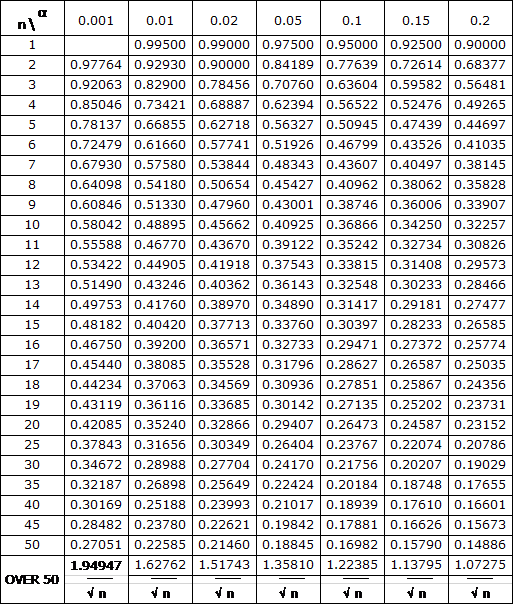
\includegraphics[width=1.0\textwidth]{./image/ks-table.png}
\end{center}
\end{figure}
\end{appendices}

\end{document}